\documentclass[conference]{IEEEtran}

\usepackage{cite}
\usepackage{tabularx}
\usepackage{amsmath,amssymb,amsfonts}
\usepackage{algorithmic}
\usepackage{graphicx}
\usepackage{textcomp}
\usepackage{xcolor}
\usepackage{multirow}

\def\BibTeX{{\rm B\kern-.05em{\sc i\kern-.025em b}\kern-.08em
    T\kern-.1667em\lower.7ex\hbox{E}\kern-.125emX}}
    
\begin{document}

\title{Are there water drops in the camera lens?}
\author{\IEEEauthorblockN{Carlo Wiesse}}

\maketitle

\section{Introduction}

Water drops adsorbed by the lens refract the light that enters the camera lens, causing image disturbance. As a result, image-based recognition algorithms fail to function normally under such conditions. Therefore, it is necessary to determine in advance whether water drops are adsorbed to prevent the misrecognition of these types of algorithms. However, droplets adsorbed by camera lenses have various sizes and shapes, making them difficult to detect.

\textbf{The task is to develop and deliver an algorithm capable of detecting whether or not there are droplets on a camera lens, using images taken with that camera only.}

\section{Data}

The provided dataset consists of 1006 images where 503 are clear and the other 503 show droplets. There are also 30 images reserved for the final evaluation, with 15 of these images being clear and the other 15 covered by droplets.

\phantom{a}

The preliminary analysis shown in Figure \ref{fig:channels} demostrates that taking only the blue channel from the provided images reduces the presence of clouds. As a blue sky and a white cloud both share a high pixel value in the blue channel, taking only the blue channel will suppress most clouds. Clouds, or in other words, white areas in the middle of a blue sky, resemble the light refracted by the camera lenses due to droplets, which would only make our task harder.

\textbf{Decision 1.} I decided to work only with the blue channel of the input images for this task.


\begin{figure}[h!]
\centering
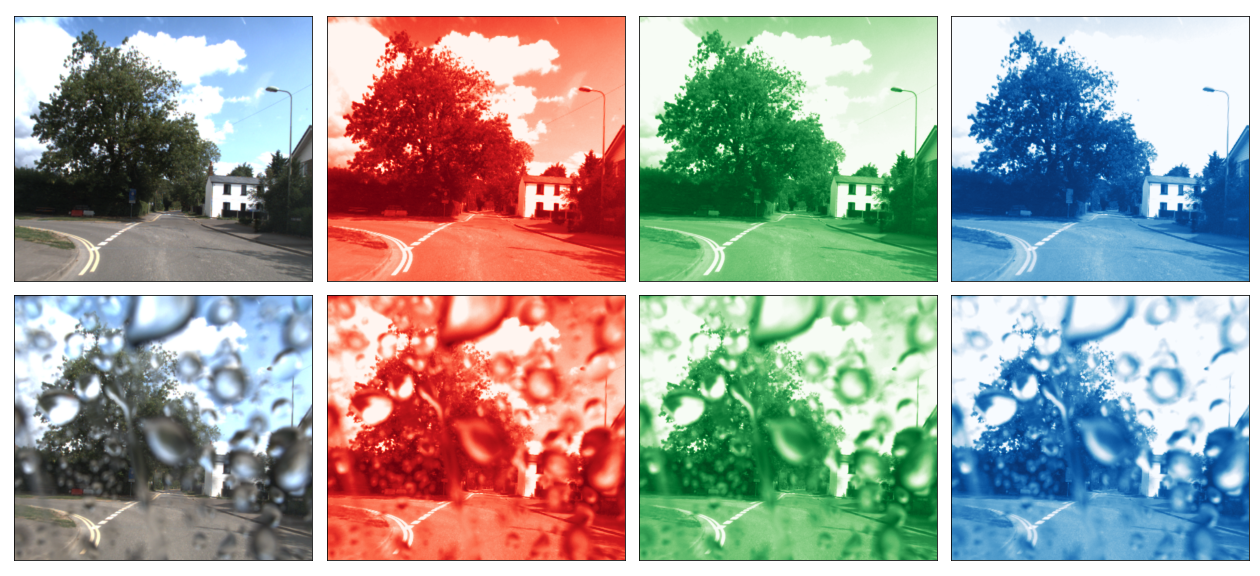
\includegraphics[width=\linewidth]{images/channels.png}
\caption{RGB input with its 3 color channels}
\label{fig:channels}
\end{figure}

Further analysis showed too much contrast between the ground and the sky, meaning we can either focus on the sky or the ground for droplet detection. For such reason, gamma correction was performed on the images to lighten the contrast. The results of this operation are shown in Figure \ref{fig:gamma}.

\textbf{Decision 2.} I decided to apply gamma correction to all input images for this task.

\begin{figure}[h!]
\centering
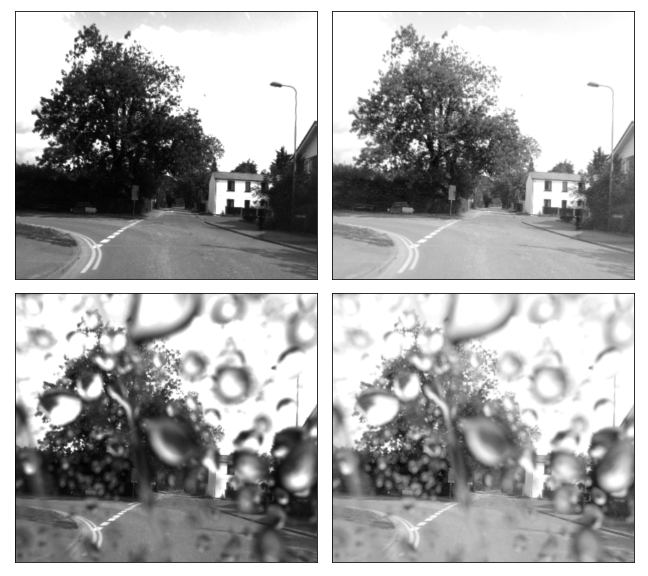
\includegraphics[width=0.87\linewidth]{images/gamma.png}
\caption{Gamma correction}
\label{fig:gamma}
\end{figure}

At the end, the pixel values of the blue channel of an input image after applying gamma correction will look as the 3D graph in Figure \ref{fig:frequency}. Here we can observe the high-frequency behavior of the droplet textures. High-frequency textures stand out in an image creating contrast, which is why we can perceive droplets so easily. As evidenced by the undulatory behavior of the pixel values on the droplet image, this seems to be the biggest difference between clear and droplet images.

\textbf{Decision 3.} I decided to extract features related to pixel frequency for my proposed approach.

\begin{figure}[h!]
\centering
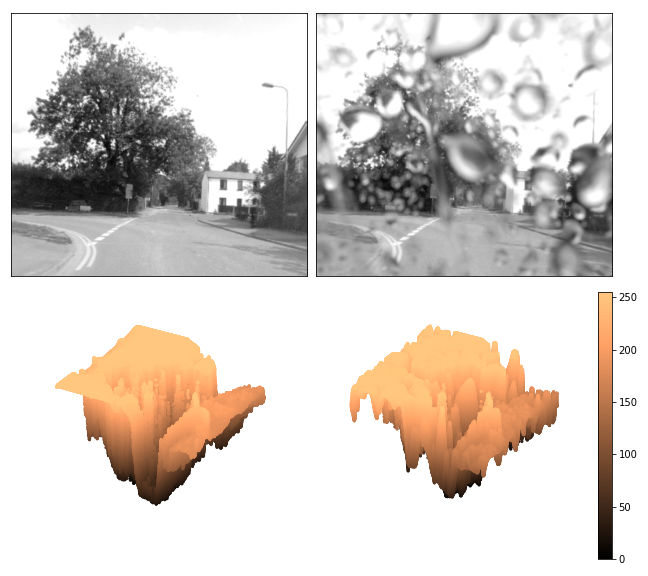
\includegraphics[width=0.87\linewidth]{images/frequency.png}
\caption{Pixel values of the preprocessed input plotted as a 3D graph}
\label{fig:frequency}
\end{figure}

\section{Solution}

\subsection{Proposed approach}
During the preliminary analysis, I realized the high-frequency behavior of the droplet textures. The best way to extract features related to frequencies is using the Fast Fourier Transform (FFT), and Gist features do just that in \cite{Oliva2001}. Therefore, this approach extracts Gist features from images and classifies these features into clear or droplet images using a Support Vector Machine (SVM).

\begin{figure}[h!]
\centering
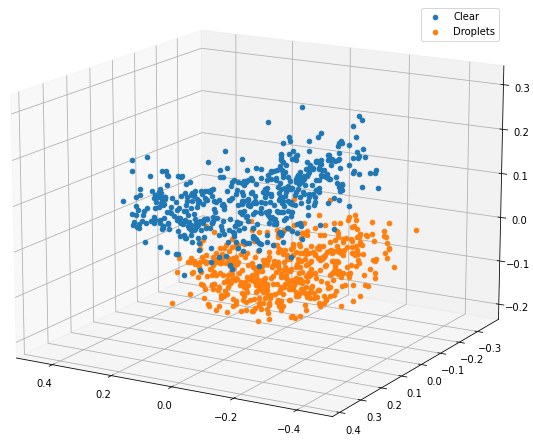
\includegraphics[width=0.9\linewidth]{images/pca.png}
\caption{Labelled feature space for all images in the training set}
\label{fig:pca}
\end{figure}

Figure \ref{fig:pca} shows a clear division between these two clouds of feature points, confirming my claim that frequency is very relevant to this task.

\subsection{Alternative approaches}

For the sake of comparison, I also opted to train a deep learning model, as they excel at identifying complex features from images. Moreover, with deep learning being so popular, likely, someone has already tried to solve the same problem or similar using this approach. Therefore, I decided to look for research papers on droplet detection and found \cite{Bae2019}, a paper on raindrop detection. This paper provides two models, one for detection and one for classification. However, the authors claimed that their detection model wasn't fit for real-time processing due to its high complexity. This situation left us with their proposed classification model, which I implemented and tested successfully.

As the raindrop detection scheme from \cite{Bae2019} was unsuitable for our task, I developed a droplet detection scheme. This alternative approach uses foreground extraction, image segmentation, and blob detection to filter out droplets in the image. Then I set a minimum number of raindrops detected as a threshold to decide whether the image is clear or not.

\section{Results}

As for the implementation details, the evaluation was performed using single-point precision (FP32) on a laptop with a 1.60 GHz Intel i5-8250U processor and no graphics card. The code is written using Python 3.6.9.

\begin{table}[h!]
\caption{Classification and computational performance results}
\begin{tabularx}{\textwidth}{|c|c|c|c|}
\cline{1-4}
\\[-1em]
\multirow{2}{*}{Metric} & \multicolumn{3}{c|}{Approach}\\
\cline{2-4}
\\[-1em]
& \textbf{Proposed} & Alternative 1 & Alternative 2\\
\cline{1-4}
\\[-1em]
Recall & 1 & 0.93 & 1\\
Precision & 1 & 0.93 & 1\\
\cline{1-4}
\\[-1em]
Computation time & 104 $\pm$ 2 ms & 406 $\pm$ 22 ms & 107 $\pm$ 2 ms\\
RAM memory used & 230 MB & 1380 MB & 230 MB\\
\cline{1-4}
\end{tabularx}
\end{table}

\subsection{Proposed Approach}

I achieved a perfect score on the training and the evaluation set, making this approach the best so far. Additionally, SVMs provide great generalization, so I'm confident this approach will work well even on images outside our dataset.

\textbf{Decision 4.} As this approach was perfect, I decided to submit the proposed approach as my solution to the task.

\subsection{Alternative approaches}

The results of the deep learning model (Alternative 1) were quite good but still failed in some cases of the evaluation set. For instance, when most image contents were light going through trees and blurry objects, the classifier may misclassify a clear image as a droplet image. So, in essence, the light going through trees gets confused with droplet refraction and blurry objects with droplet texture. On the other hand, droplet texture merges with the trees and road when the image is mostly forest and road with little to no light from the sky. As the characteristic droplet refraction becomes less evident, the classifier may perceive droplet images as clear.

As for the other approach (Alternative 2), this proved to be very successful, even achieving a perfect score in the evaluation set. However, it required extensive parameter tuning, making this approach very sensitive to changes in the dataset.

\section{Conclusions}

Finally, given how crucial it is to know when images become unusable for other visual algorithms, I would focus on recall. A high recall means fewer misclassifications, while high precision means fewer false alarms. Therefore, a high recall would be my priority to ensure droplets are always detected, which won't be a problem based on my results. The proposed approach shows great performance in terms of classification, generalization capabilities, and computation time.

So far, I'm unaware of the limitations of this approach since it worked flawlessly with all the training and evaluation data. However, images with only small droplets or those with droplets clustered on the camera lens border may require tuning the Gist feature extraction parameters.

\bibliographystyle{apalike}
\bibliography{bibliography.bib}

\end{document}
